%  Introduction.tex
%  Document created by seblovett on seblovett-Ubuntu
%  Date created: Sun 16 Feb 2014 09:18:38 GMT
%  <+Last Edited: Sat 22 Mar 2014 12:19:33 GMT by seblovett on seblovett-Ubuntu +>
% !TeX spellcheck = en_GB
% !TeX root = Report.tex
\phantomsection
\addcontentsline{toc}{section}{Introduction}
\sect{Introduction}

%\inote{Needs some neatening and completing. More references! Definition of terms done}

Starting a company is a very difficult task to undertake. 
There is much discussion as to the strategy that should be taken in order to make the company successful \cite{hsu2006venture,smith1997utility}.
In this report, an emerging company is one which has been around for eight years or less \cite{zahra1996technology}. 
An emerging company is deemed successful if it then becomes an established company after the 8 year mark.
An established company is one where the company has developed a product range for a specific market \cite{kekale2007successful}.
It can also be successful if it is acquired by and/or merged into an established company. 

%\inote{Discussion of patents, how to acquire, costs, why, benefits, drawbacks\dots Should fill the rest of the intro}
A patent is legal protection over an invention.
They cover how things work, their operation and their manufacture. 
According to \cite{ipopatent}, a patent must be:
\begin{itemize}
\item a new and novel idea
\item an inventive step that it not obvious to an expert in the relevant field
\item manufactured or used in an industry
\end{itemize}

As well as this, \cite{ipopatent} says a patent cannot be:
\begin{itemize}
\item a mathematical or scientific theory, discovery or method
\item dramatical, musical, literary or artistic discovery
\item presentation of information, or some computer programs
\item an animal or plant vareity
\item a method of medical diagnosis or treatment
\item immoral or against public policy
\end{itemize}

%\todo[inline]{Reasons to patent}

Valid patents provide the holder ``an `absolute' monopoly'' over their invention for 20 years \cite{waelde2013contemporary}.
This is the main advantage to own a patent as it results in other companies being unable to copy your idea to undermine the patent holder.
This exclusivity can also increase the value in a company, and established companies may wish to purchase and merge to acquire the intellectual property of a company.
An example of this is Atmel's acquisition of Quantum Research Group to acquire IP around touch screen technology \cite{atmel:acq:qrg08}.
This gave Atmel a quick start in this market.% \cite{NEEDED}. \todo[color=green!40]{Find citations of company acquisitions for IP. QRG?}
Patents themselves can also be licensed or sold in the case that they are not exploited by the patent holder. 

%\todo[inline]{Reasons not to patent}
Patents can typically cost between \pounds 230 - \pounds 280 to file. 
Renewal costs are then between \pounds 70 and \pounds 600 depending on the age of the patent \cite{ipocosts}.
The technology patented must earn more money that it costs to hold the patent, else it looses the patent holder money.
However, holding a patent is one aspect of the costs - there are also the costs involved in defending your patents.
This mainly includes the legal fees involved in taking the accused to court. 
Therefore a company must be in a strong financial situation to be able to hold and successfully defend a patent; a luxury that can not always be exercised by an emerging company.


There is a long running debate around whether computer programs and algorithms can be patented \cite{juden2005can, klemens2005math}.
An algorithm can be seen as a mathematical method, which violates the IPO's rule for patents.
However, in the USA, there are no such restrictions, and allow a ``new, non obvious and useful'' process to be patented \cite{usapatent}.
\todo[inline,color=red]{Is the above needed?}

In \cite{zahra1996technology}, a six stage plan for an emerging company is discussed. 
Although this is aimed at the biotechnology industry, the strategy still applies to other areas. 
The later parts of the strategy concern the research and development, and in particular, the acquisition of patents. 


This report aims to investigate whether the early acquisition of patents leads to the success of an emerging company.
Four possible combinations have been identified and depicted in figure \ref{fig:synergymatrix}. 
A company can either acquire patents early, or later on. 
The company can then be either a success or a failure as previously defined.

\begin{figure}
\centering
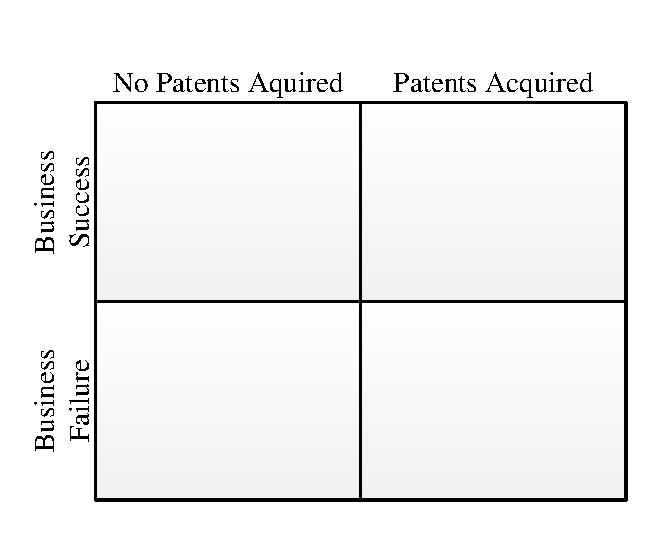
\includegraphics[width=0.5\textwidth]{./Figures/SuccessMatrix.pdf}
\caption{Patent-Success Synergy Matrix}
\label{fig:synergymatrix}
\end{figure}

The report is spit into three sections. 
The first discusses material from the invited talks, with thought to the report's hypothesis.
The second documents a number of case studies investigating the hypothesis.
The final section then concludes the report.
